\Subsection{Datastrukturer}

\Subsubsection{node}
En länkad lista används för att implementera en stack. I det här programmet behövs en stack för att
spara dom mappar som programmet ska söka i, kallad \texttt{taskpool}.

\Subsection{Viktiga variabler}

\Subsection{Funktioner}
\Subsubsection{int main(int argc, char *argv[])}
Läser in argument och initialiserar mutexar och variabler. Huvudtråden ser till att de andra trådarna
kör \texttt{taskManager}. Huvudtråden kör sedan också \texttt{taskManager}. När alla trådar är klar med \texttt{taskManager} så städar huvudtråden upp och programmet avslutas.

\Subsubsection{void * taskManager(void *pArg)}
Hanterar synkroniseringen mellan trådarna. Det som i slutändan görs är att kalla \texttt{mfind\_p}
tills alla mappar som ska sökas igenom; har blivit genomsökta.

\Subsubsection{void mfind\_p(char *path, pcre *find, int type)}
Kollar upp alla filer i gen givna mappen på \texttt{path}. Ifall filen är den som söks---d.v.s. den är av typen \texttt{type} och passar det reguljära uttrycket \texttt{find}---så skrivs sökvägen
ut på standard output. Ifall filen är en mapp men inte "." eller ".." så sparas den i stacken (\texttt{taskpoolen}) för att någon tråd ska kunna använda den som argument i \texttt{mfind\_p}. 

\Subsubsection{void read\_arguments(int argc, char *argv[], par\_t *par)}
Tolkar inargument och verifierar att dom är på rätt format.

\Subsubsection{char * popTask(void)}
Tar bort den mapp som ligger högst upp i stacken från stacken(\texttt{taskpoolen}) och returnerar den.

\Subsubsection{void pushTask(char* v)}
Lägger till en mapp till stacken (\texttt{taskpoolen}).

\Subsection{Anropsdiagram}
\begin{figure}[h!]
	\centering
	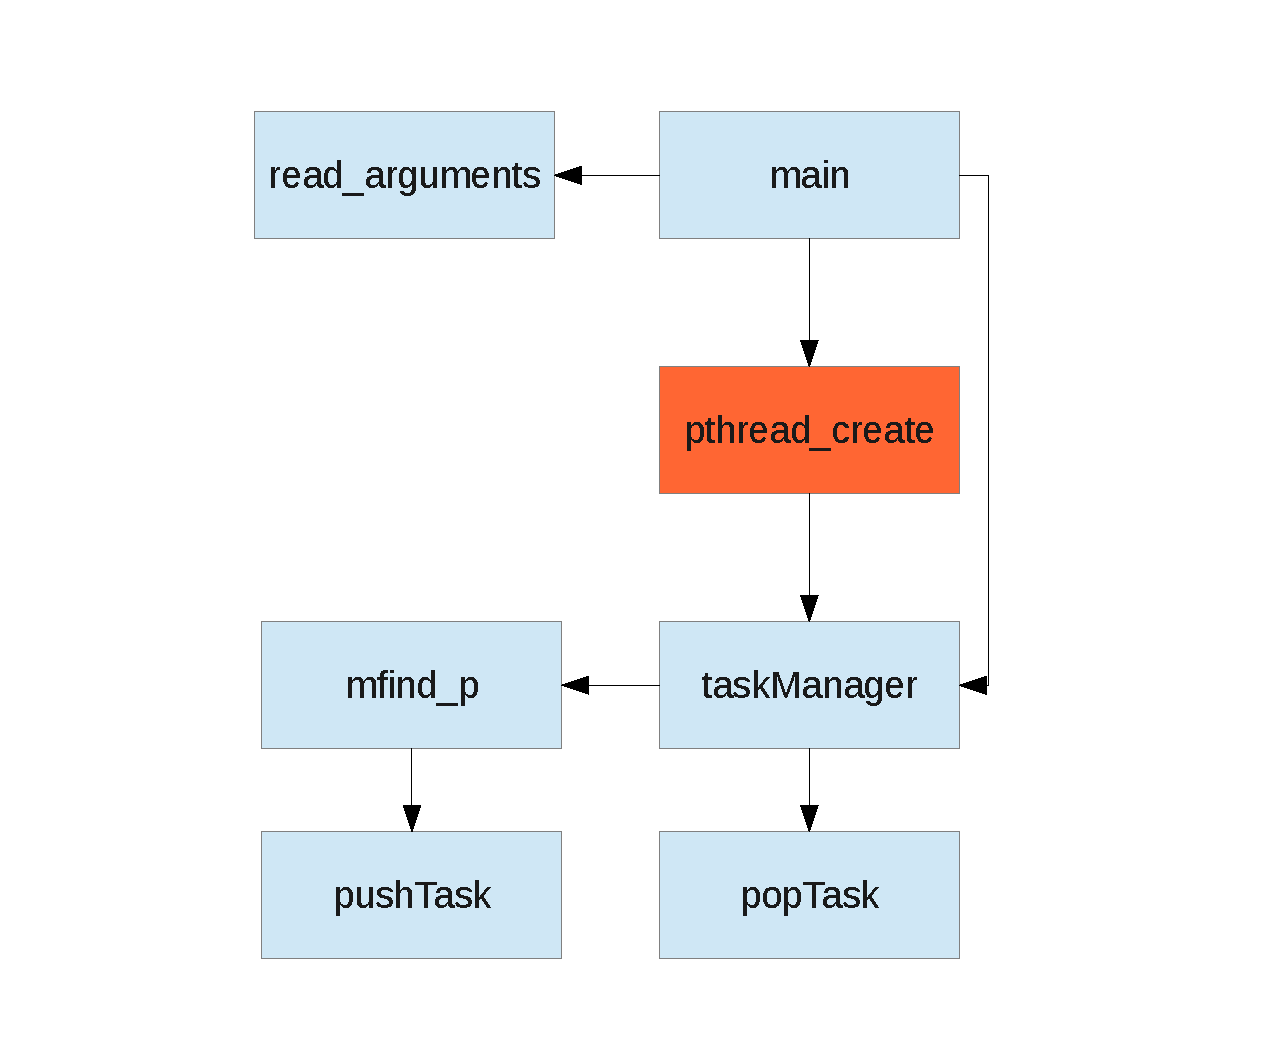
\includegraphics[width=0.8\textwidth]{img/anropsdiagram}
	\caption{Anropsdiagram för programmet mfind\_p.}
	\label{fig:anropsdiagram}
\end{figure}
